\documentclass[11pt, a4paper]{article}
\usepackage[utf8]{inputenc}
\usepackage{geometry}
\usepackage{graphicx}
\usepackage{float}
\usepackage[dvipsnames]{xcolor}
\geometry{margin=1in}
\setlength{\parindent}{0em}
\setlength{\parskip}{1em}
\title{Computação Gráfica | Trabalho 3}
\author{Professor: Waldemar Celes\\
Aluno: Antenor Barros Leal}
\date{01 de dezembro de 2024}
\begin{document}
\maketitle

\section {Resumo}
Este trabalho tem como objetivo fazer a implementação e teste de técnicas de renderização
em uma cena 3D.

\section {Cena Base}
Para a cena utilizou-se uma versão com leves modificações a partir da tarefa 2.1. 
A cena base é a seguinte:

\begin{figure}[H]
  \begin{center}
  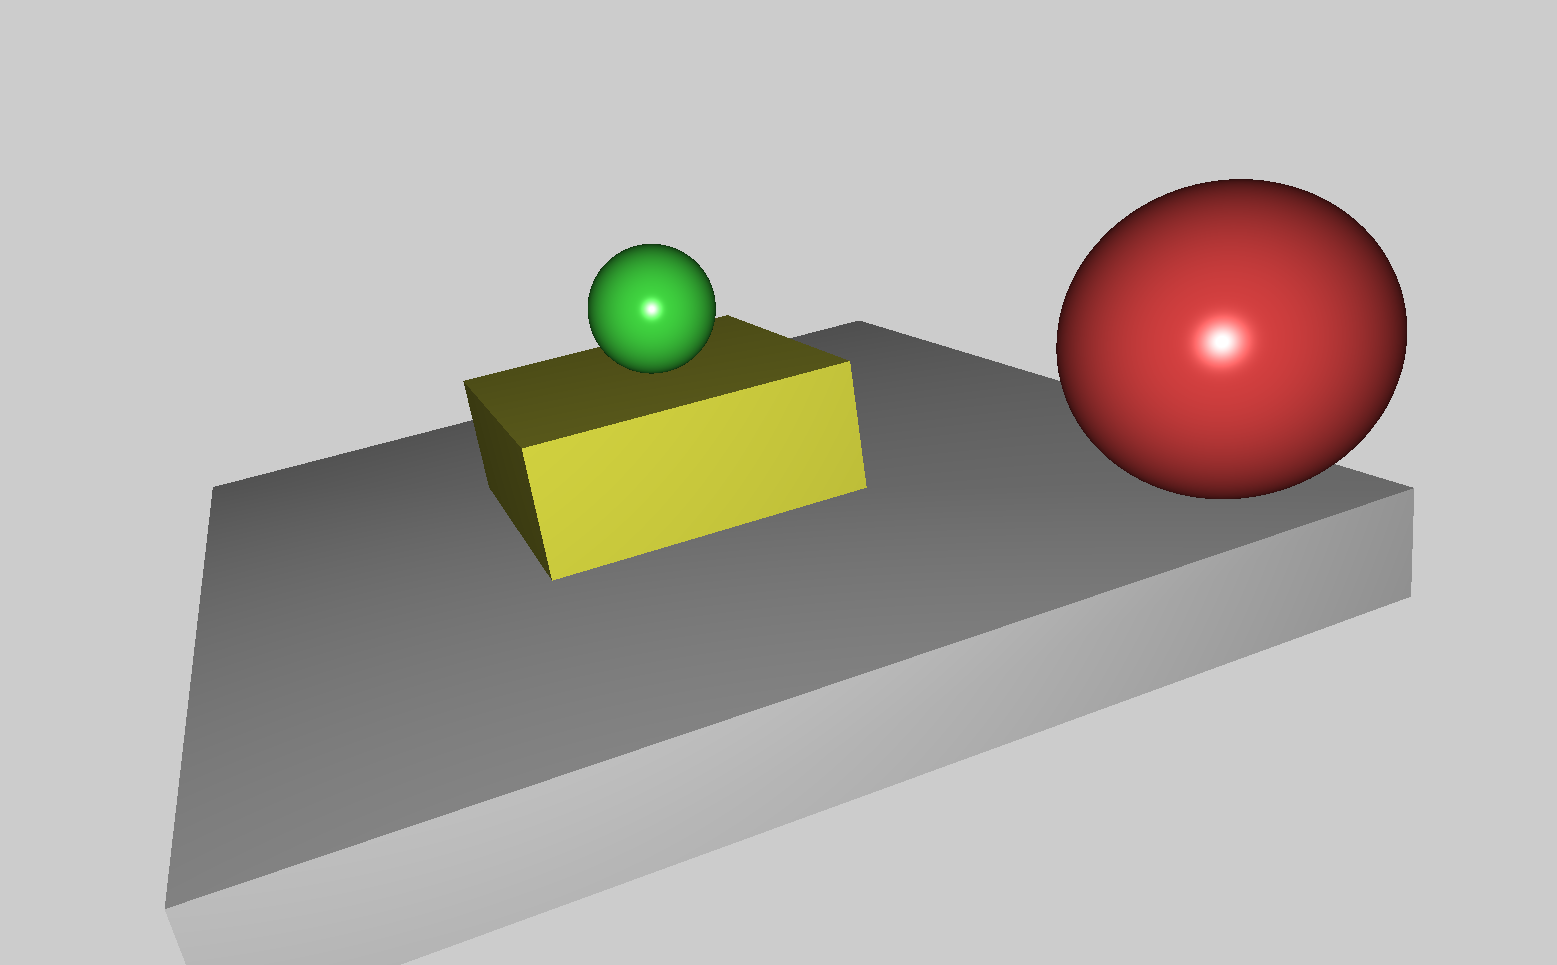
\includegraphics[width=0.8\linewidth]{base-scene.png}
  \caption{Cena base}
  \label{fig:cena-base}
  \end{center}
\end{figure}

Para este trabalho o cubo cinza foi retirado para ser substituído por um quad 
que fará papel de uma superficie plana para o refletor.

O seguinte grafo de cena foi usado:

\begin{verbatim}
  Node::Make(shader,
      {
      Node::Make(trCube2,{yellow},{cube}),
      Node::Make(trSphere1,{green},{sphere}),
      Node::Make(trSphere2,{red},{sphere}),
      }
  );
\end{verbatim}

\section {Técnicas de Renderização}

Entre as opções, foi escolhido a técnica de reflexão planar e de sombra planar.

\subsection {Técnica: reflexão planar}

Como dito na seção anterior foi usado um quad para receber a reflexão que é 
simplesmente a repetição da cena em $$y > 0$$ em $$y < 0$$ com a componente y
com sinal trocado.

\begin{verbatim}
trf->Scale(1.0f,-1.0f,1.0f);
\end{verbatim}

Todavia, se apenas isto for feito, a reflexão irá "vazar" para fora da superficie
reflexiva.

\begin{figure}[H]
  \begin{center}
  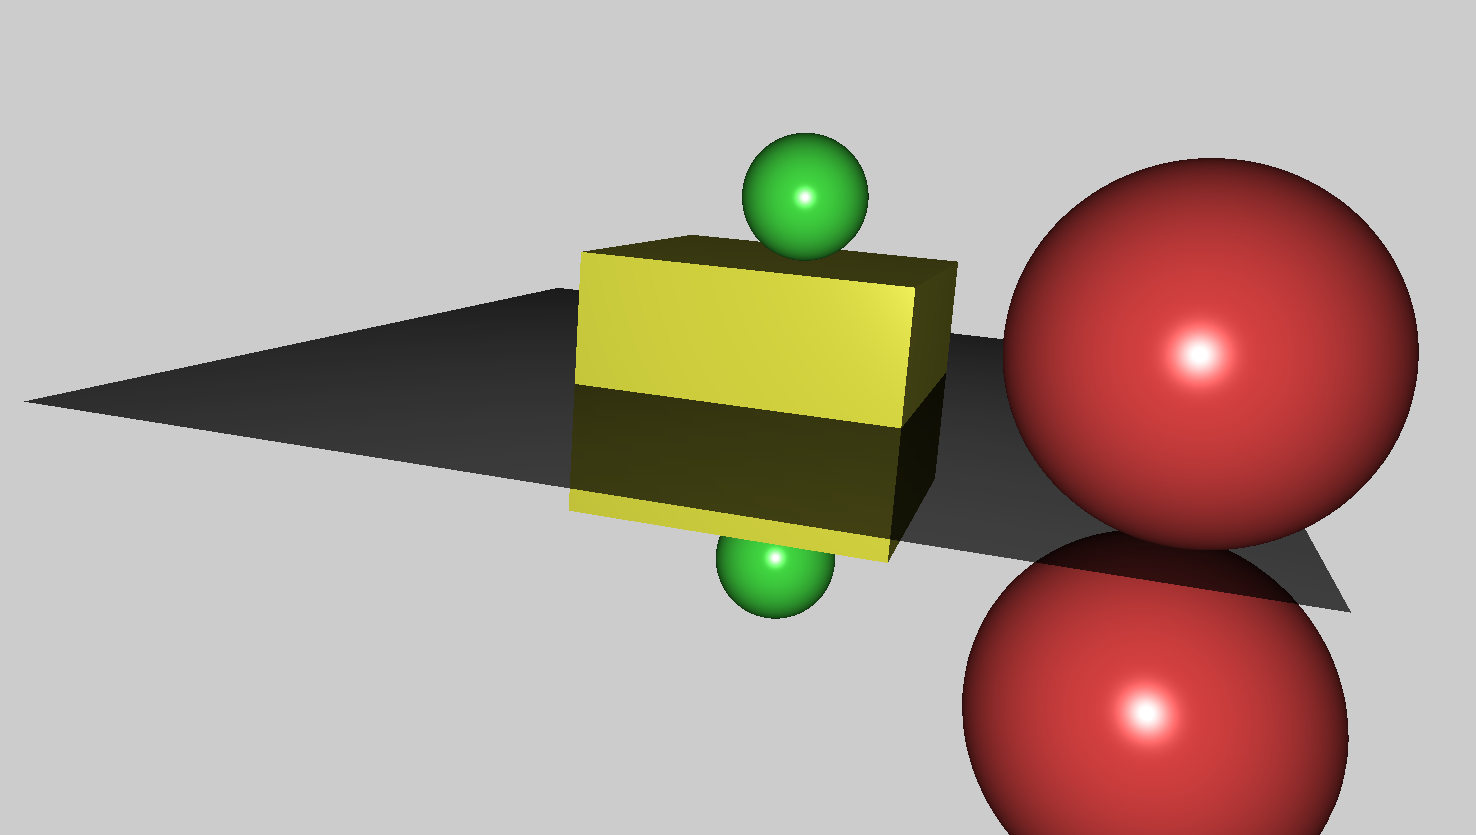
\includegraphics[width=0.8\linewidth]{before-stencil.png}
  \caption{Antes do stencil}
  \label{fig:vaz}
  \end{center}
\end{figure}

Isto é resolvido aplicado um stencil na superficie reflexiva e informado ao 
ao OpenGL não rederizar a reflexão que esteja fora desta máscara.

\begin{figure}[H]
  \begin{center}
  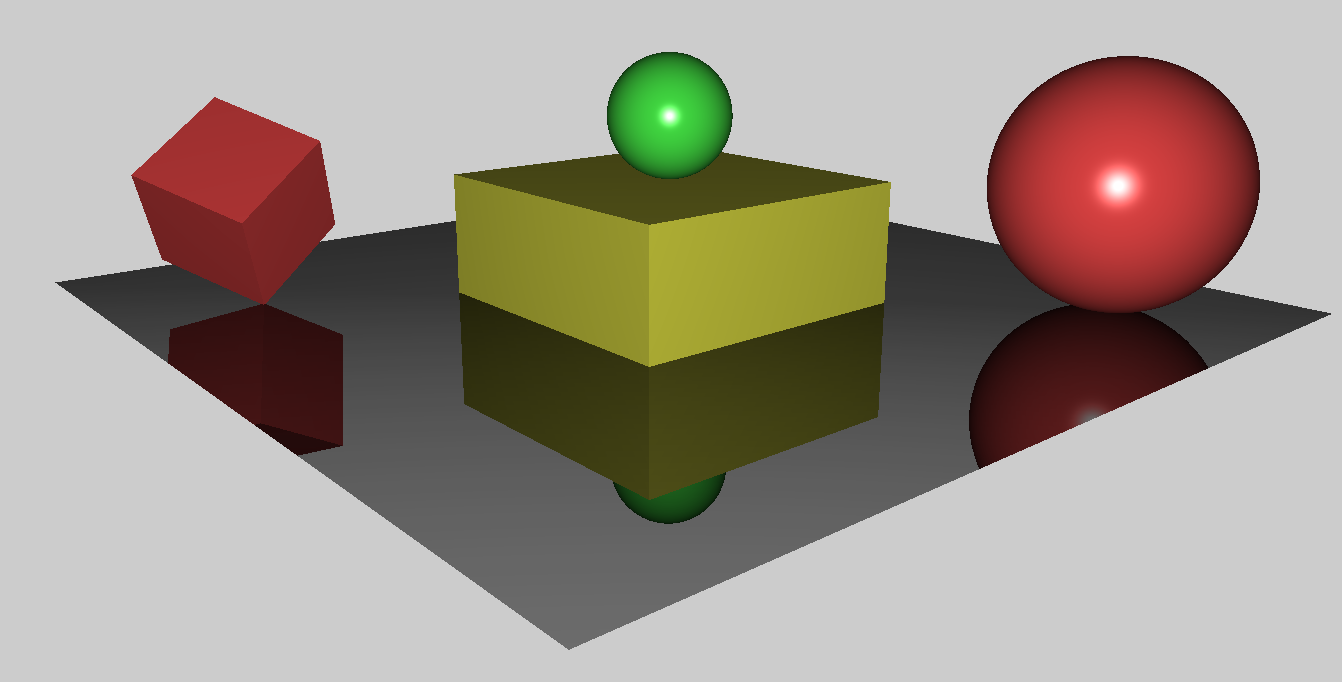
\includegraphics[width=0.8\linewidth]{after-stencil.png}
  \caption{Depois do stencil}
  \label{fig:vaz}
  \end{center}
\end{figure}

Porém se mudarmos o arcball para visualizar a parte de baixo da superficie reflexiva, 
vemos parte do reflexo cortado pelo stencil. O que se é desejado, obviamente, é 
a ausencia de qualquer objeto.

\begin{figure}[H]
  \begin{center}
  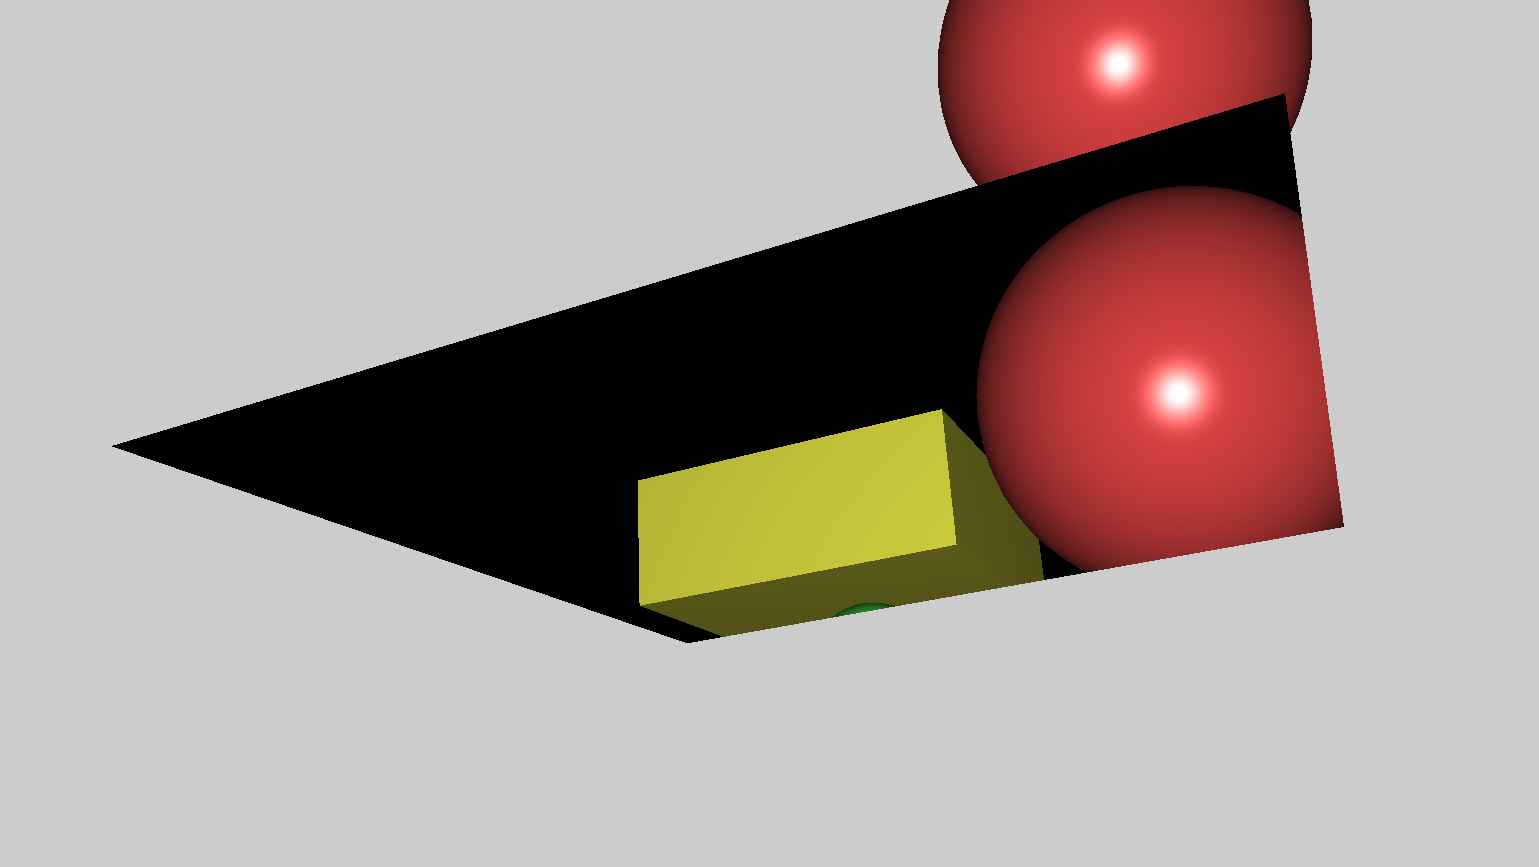
\includegraphics[width=0.8\linewidth]{before-cut-plan.png}
  \caption{Antes do plano de corte}
  \label{fig:vaz}
  \end{center}
\end{figure}

Para resolver isso usamos um plano de corte para mostrar a cena refletida apenas
acima do plano de corte.


\subsection {Técnica: sombra planar}

Para a sobra planar aplicamos a geometria em uma matriz de projeção que "achata"
os objetos de cena em uma superficie 2D. Esta matriz de projeção por considerar a posição da luz
conseguie simular corretamente como é a sombra projetada por esta luz.

\section {Resultados}

Além das capturas de tela deste relatório, um vídeo de demostração do funcionamento 
foi incluído: arquivo "demo.mp4".

\end{document}